%Usually an article, 12pt font, with a separate title page
\documentclass[12pt]{article}
\usepackage{preamble}
\usepackage{csvsimple}

\begin{document}

% Edit title page in the titlepage.tex file.
% This title page template belongs to Apex Automation and may not be used without their consent.



% Please fill out the following information.
\newcommand{\org}{McMaster University}   % Enter name of organization
\newcommand{\headingmajor}{MECHTRON 4TB6A}   % Enter the major heading
\newcommand{\headingminor}{Mechatronics \& Software Engineering Capstone}   % Enter the minor heading
\newcommand{\doctitle}{System Requirements}   % Enter the title of the document
\newcommand{\projtitle}{Health Mate - Pill Dispenser}   % Enter the project title
\newcommand{\logofile}{ApexEngineering.png}   % Enter the file name for team logo
\newcommand{\projdate}{Sunday, November 1, 2020}   % Enter the date



%--------------Do not touch below this line unless you intent to change format, spacing, etc.-----------------
\begin{titlepage}

% Defines a new command for the horizontal lines, change thickness here
\newcommand{\HRule}{\rule{\linewidth}{0.5mm}}

% Center everything on the page
\center

% HEADING SECTIONS
\textsc{\LARGE \org}\\[1.5cm] % Name of your university/organization
\textsc{\Large \headingmajor}\\[0.5cm] % Major heading such as course name
\textsc{\large \headingminor}\\[0.5cm] % Minor heading such as course title

% TITLE SECTION
\vspace{1cm}
\HRule \\[0.2cm]
{ \Large \vspace{0.25cm}  \textsc{  \LARGE \doctitle} \vspace{0.3cm} }  % Title of your document
\HRule \vspace{.5cm}
\textsc{\LARGE \projtitle} % Project title
\vspace{1cm}
% Firm/Team logo included here. 
 \begin{figure}[h]
  \centering
  \includegraphics[width=.4\linewidth]{\logofile}
\end{figure}
 \vspace{1cm}
 
% AUTHOR SECTION
\begin{table}[ht!] \centering
\begin{tabular}{c c c}
\toprule
\textbf{Name} & \textbf{Student Number} & \textbf{McMaster Email} \\ 
\midrule
Justin Ballaro & 400015482 & ballaroj@mcmaster.ca \\
Joel Bates & 001420696 & batesjj@mcmaster.ca \\
Brodie Bresette & 400029059 & bresettb@mcmaster.ca \\
Nicholas D'Angelo & 400018631 &  dangelon@mcmaster.ca  \\
Daniel Pietrangelo & 400010287 &  pietrand@mcmaster.ca \\
\bottomrule
\end{tabular}
\label{Tab:HU}
\end{table}

% DATE SECTION
%{\large \projdate}\\[3cm] % Date exlcude b/c it is available in the revisions table.
\end{titlepage}
 
\pagebreak
% header and footer settings
\pagestyle{fancy} \fancyhf{}
\lhead{\fontsize{10pt}{10pt}\selectfont System Requirements} \rhead{\fontsize{10pt}{10pt}\selectfont Revision \rev} \cfoot{\thepage}

% Edit table of revisions in tableofrevisions.tex
\pagenumbering{roman}


\newcommand{\rev}{0}  %-------INSERT MOST RECENT REVISION NUMBER HERE

\section*{Table of Revisions}
\begin{table}[ht!]
\begin{center}
\begin{adjustbox}{max width=\textwidth}
\small
\begin{tabular}{|p{0.1\textwidth}|p{0.15\textwidth}|p{0.2\textwidth}|p{0.4\textwidth}|}
 \hline
 \textbf{Revision } & \textbf{Date} &
 \textbf{Authors} &
 \textbf{Revision Comments}\\
 \hline \centering
 0 & \centering
 17/02/2021 & 
 Justin Ballaro \newline
Joel Bates \newline
Brodie Bresette \newline
Nicholas D'Angelo \newline
Daniel Pietrangelo &
Inital Revision \\
\hline
\end{tabular}
\end{adjustbox}
\end{center}
\caption{Table of Revisions}
\end{table}

\pagebreak
\tableofcontents
\listoffigures
\listoftables
\pagebreak
\pagenumbering{arabic}

%----------Begin adding text here.----------
\section{Introduction}
% \subsection{Scope of Project}
% The desired system shall automate the dispensing of a person's medication from a standard sized pill blister back that is inserted by the user. This dispensing shall occur at times set by the user within the specified ranges of the pill blister pack (Morning, Afternoon, Evening, Night). The device shall also collect dispensing statistics for review by the user along with any other health professional. 

\subsection{Scope of Document}
The scope of this document is to outline potentially hazardous issues that could result from the pill dispenser's software and hardware subsystems.

The scenarios outlined in this document will be constructed from cases where the device is functioning correctly in normal operation as well as cases where the device is considered to be functioning incorrectly. Also, hazards that could potentially evolve from the development of this device will be analyzed and included in this report. This analysis should be conducted throughout the development life cycle of the device. 



\section{System Overview}

\noindent An overview of the system can be found in the context diagram below. All system components are contained within the red box of the diagram. Descriptions of each component can be found below.


\begin{figure}[H]
    % \centering
    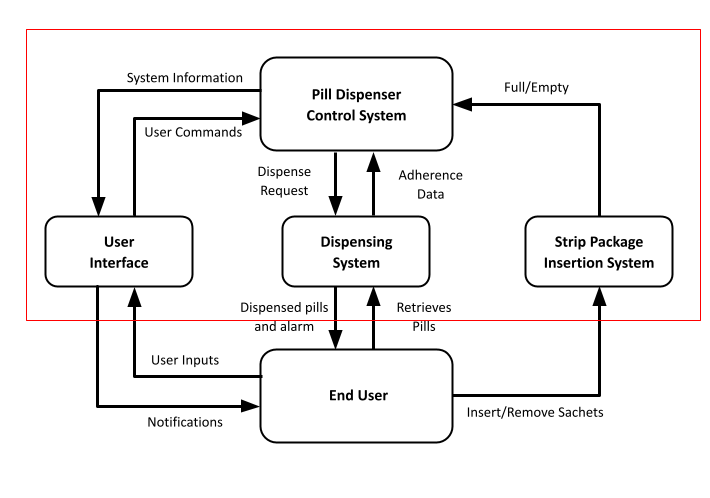
\includegraphics[width=\textwidth,height=\textheight,keepaspectratio]{./ContextDiagram-HazardAnalysis.png}
    \caption{Context diagram - component overview}
    \label{fig:my_label}
\end{figure}


\subsection{Pill Dispenser Control System}
Consists of the finite state machine of the system along with the device's back-end. Sub-components of this system include: Scheduling system, Notification system, Calibration System, Data Collection System. 
\subsection{Dispensing System}
The dispensing system for the device will perform the required motion to successfully deliver the pouches to the dispensing area. This system also includes the mechanism for cutting the pouches open for the user.
\subsection{User Interface}
The user interface will be the point of interaction to the device for the user. This system consists of a on-device touchscreen.
\subsection{Strip Package Insertion System}
This system will allow the user to load the desired strip package into the device.

% \subsection{Scheduling System}
% This system allows the user to set a dispensing time for each dispensing period (Morning, Afternoon, Evening, Night).
% \subsection{Notification System}
% The device's notification system will alert the user when the time has been reached to take their scheduled medication. This includes an audible alarm, a visual queue on the device's display, as well as a flashing light.
% \subsection{Loading System}
% This system will allow the user to load the desired strip pack sachet into the device.
% \subsection{Calibration System}
% The calibration system will ensure the strip pack sachets are loaded properly into the device, all system parameters are set correctly and the dispensing mechanism is in working order. 
% \subsection{Dispensing System}
% The dispensing system for the device will perform the required motion to successfully deliver the sachets allowing the pills to be retrieved from the dispensing area. This system also includes the mechanism for pill retrieval.
% \subsection{Data Collection System}
% Data collection for the device will involve collecting on-board sensor data to retrieve metrics on medication adherence and device use. 

\section{Safety Considerations}

\noindent \textbf{Note:} If a system consists of a set of subsystems (e.g. Pill Dispenser Control System), all hazards will be categorized based on the related subsystem.

\subsection{Pill Dispenser Control System}
\subsubsection{Scheduling System}
\subsubsection*{Software Issues}
\begin{itemize}
\item Schedule file corruption during saving or loading to/from device.
\item Scheduling system timing configuration may not match the time used on the device. This may cause conflict of timing between the device and schedule.
\item Dispensing time scheduled that is outside allowable range of values.
\item Previously inputted schedule could be lost due to override of new schedule.
\end{itemize}
\subsubsection*{Hardware Issues}
\begin{itemize}
% \item Mechanism for user input malfunctions (faulty connection, touch screen).
\item Display used to set schedule malfunctions.
\end{itemize}

\subsubsection{Notification System}
\subsubsection*{Software Issues}
\begin{itemize}
\item Notification signal is not sent/is sent at the wrong time (in accordance with scheduling system).
\item Notification signal is not terminated once pouch are retrieved from the device.
\item Notification signal is terminated before pills are retrieved or before time-out duration is reached.
\end{itemize}
\subsubsection*{Hardware Issues}
\begin{itemize}
\item Alarm/Speaker stops working or burns out.
\item If accuracy or reliability of on-board RTC is not sufficient, notifications may not be triggered.
\item Display used to terminate alarm malfunctions.
\end{itemize}

\subsubsection{Calibration System}
\subsubsection*{Software Issues}
\begin{itemize}
\item Calibration signal is not received from hardware.
\item System detects a successful calibration as a failure and vice versa.
\end{itemize}
\subsubsection*{Hardware Issues}
\begin{itemize}
\item Limit sensor fails to actuate.
\item Limit sensor is not sending electrical signal (loose connection, faulty parts)
\item Dispensing mechanism damages limit sensor.
\end{itemize}

\subsubsection{Data Collection System}
\subsubsection*{Software Issues}
\begin{itemize}
\item Corruption of data when saving/loading to and from device.
\item Failure to record taken and missed medication doses.
\item False negative and false positive data is recorded for taken/missed dose.
\item Failing to write data into non-volatile memory.
\end{itemize}
\subsubsection*{Hardware Issues}
\begin{itemize}
\item Memory controller fails to receive read/write signal.
\item Memory controller fails preventing further reads \& writes.
\end{itemize}

\subsection{Dispensing System}
\subsubsection*{Software Issues}
\begin{itemize}
\item System does not dispense medication at the scheduled time.
\item Signal to dispense is sent to system when a pill strip package is not loaded into the device.
\item Signal to dispense is sent to system before a successful calibration has taken place.
\item Manual request dispense signal fails to reach internal mechanism.
\end{itemize}
\subsubsection*{Hardware Issues}
\begin{itemize}
\item Stepper motor not functioning properly, not ending in the proper location.
\item Failure to sense when pill pouch is dispensed.
\item System identifies a successful dispense despite there being a failure.
% \item Manual dispensing button malfunctions.
\item Insufficient power transferred from motor.
% \item Linear actuators break/becomes stuck. 
\item Pill pouch roller breaks/malfunctions.
\item Roller damages pills or pill pouch.
\item Pouches become stuck/damaged while falling into collection bay.
\item Pouches do not land in collection bay.
\item Device does not return to safe state after an unexpected power outage.
\item Unexpected obstacles preventing regular motion of motors.
\end{itemize}



\subsection{Strip Package Insertion System}
\subsubsection*{Software Issues}
\begin{itemize}
\item Device may fail to trigger signal if the pill package is correctly loaded in.
\end{itemize}
\subsubsection*{Hardware Issues}
\begin{itemize}
\item Loading system may lock/unlock during device processes when it is not needed.
\item Pill pouch becomes damaged during loading by user.
\item Pill strip package is loaded into the device in the wrong orientation.
\item Dispensing mechanisms get jammed, preventing the insertion or removal of pill strip package.
\end{itemize}

\pagebreak
\section{Failure Modes and Effect Analysis Table}


\begin{figure}[!htbp]
    % \centering
    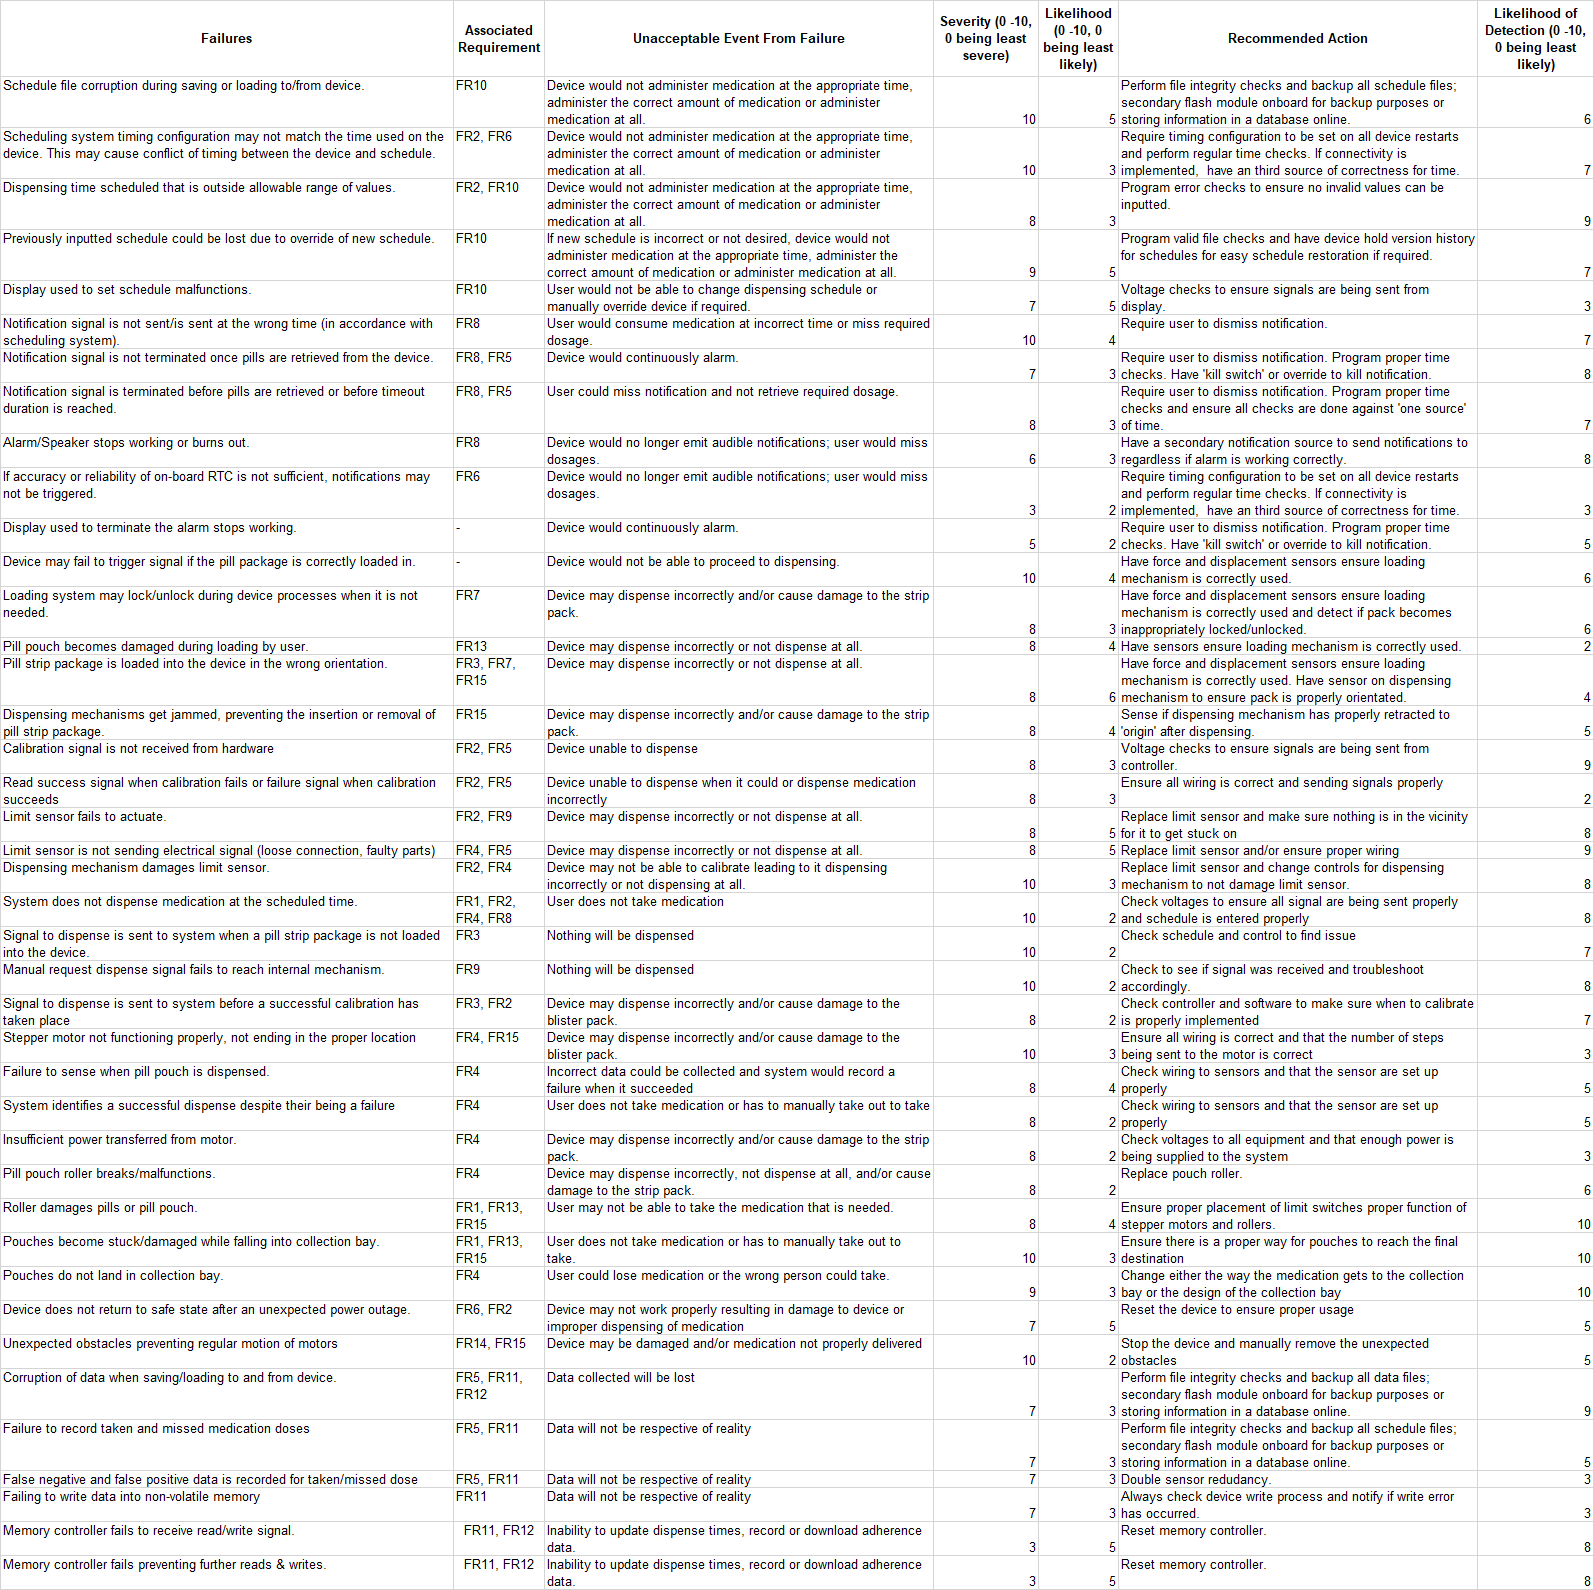
\includegraphics[width=\textwidth,height=\textheight,keepaspectratio]{./FMEA.png}
    \caption{FMEA Table}
    \label{fig:my_label}
\end{figure}



\end{document}

